\documentclass[14pt]{beamer}
\usepackage{amsmath,amssymb}

% from http://www.hartwork.org/beamer-theme-matrix/
\usetheme{default}
\usecolortheme{dove}
\beamertemplatenavigationsymbolsempty 
\setbeamertemplate{frametitle}[default][center]

% http://www.tug.dk/FontCatalogue/augie/
% \usepackage{emerald}
% \usepackage[T1]{fontenc}

% \usepackage{fontspec}
% \setmainfont{xkcd}
%
% http://kevin-keraudren.blogspot.co.uk/2014/03/xkcd-style-beamer-presentation-latex.html

\usepackage{tikz}
\usetikzlibrary{arrows,trees}

\newcommand\m[1]{\mathbb { #1 }}
\newcommand\p[1]{\mathcal{ #1 }}
\newcommand\N{\ensuremath{\m N}}
\newcommand{\cupdot}{\mathbin{\mathaccent\cdot\cup}}


\title{4-valued coalgebraic modal logic}
% \subtitle{}

\author{Tom\'a\v s~Jakl}

% \institute[KAM MFF]{
% Department of Applied Mathematics (KAM) \\
% Charles University in Prague
% }
\date[2015]{
28 January 2015
}

\newcommand{\theName}{
    \frame{
        \begin{center}
        \Large{4-valued coalgebraic modal logic}
        \vspace{4.0em}
        \end{center}
    }
}


\begin{document}
\frame{\titlepage}

\theName

\begin{frame}{4-valued logics}
    \begin{columns}
    \column{.3\textwidth}
        \begin{enumerate}
            \item true
            \item false
            \item \only<2->{$\bot$}
            \item \only<3->{$\top$}
        \end{enumerate}

    \column{.7\textwidth}
        \only<2> {
            \begin{block}{$\bot = $ Not enough information}
                \begin{itemize}
                    \item At the beginning of a computation.
                    \item Program hangs (example: trying to evaluate halting problem).
                \end{itemize}
            \end{block}
        }


        \only<3> {
            \begin{block}{$\top = $ Inconsisten information}
                \begin{itemize}
                    \item Obtained information from database don't make any sense.
                    \item Different threads returning contradicting results.
                \end{itemize}
            \end{block}
        }

        \only<4> {
            \begin{center}
            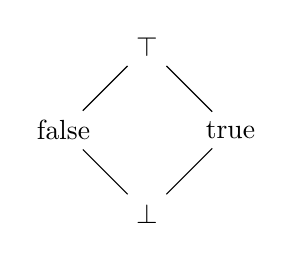
\begin{tikzpicture}[node distance=1.5cm]
            % \node[circle,draw] (T) {$\top$};
            \node (T) {$\top$};
            \node (L) [below left of=T] {false};
            \node (R) [below right of=T] {true};
            \node (B) [below right of=L] {$\bot$};

            \path (T) edge (L) edge (R)
                  (R) edge (B)
                  (B) edge (L);
            \end{tikzpicture}
            \end{center}

            \begin{align*}
                \text{true}\sqcup \text{false} = \top\\
                \text{true}\sqcap \text{false} = \bot
            \end{align*}
        }
    \end{columns}
\end{frame}

% four-valued logic solved
\theName


\begin{frame}{Modal logics}
    {\LARGE $$ s\,\models\, \Box \varphi$$}

    Starting in the state $s$, the proposition $\varphi$ is going to hold \emph{after one step of a computation}.
    \pause % with arrows
\end{frame}


% modal logic solved
\theName

\begin{frame}{What are coalgebras?}
    \begin{block}{Simple answer:}
    They are just algebras in the opposite category.
    \end{block}

    \begin{block}{More useful answer:}<2>
        Any state based system is a coalgebra. For example
        \begin{itemize}
            \item streams of bytes, single thread computation,
            \item concurrent computation,
            \item complex inteligent networks (brain, internet, finantial systems),
            \item \dots
        \end{itemize}
    \end{block}
\end{frame}

\begin{frame}{Coalgebras}
    {\large $$\sigma\colon S\to T(S)$$}

    \begin{itemize}
        \item<2-> Printing coalgebra ($T(S) = A$):
            \begin{align*}
                \sigma\colon S&\longrightarrow A\\
                \sigma\colon s\in S&\longmapsto \sigma(s)\in A
            \end{align*}
        \item<3> Changing-states coalgebra ($T(S) = S$): 
                $$\sigma\colon S\longrightarrow S$$
    \end{itemize}
\end{frame}

\begin{frame}{Coalgebras of combined shapes}
    \begin{itemize}[<+->]
        \item Choice: $$\sigma\colon S\to T_1(S) \cupdot T_2(S)$$
        \item Parallel composition: $$\sigma\colon S\to T_1(S) \times T_2(S)$$
            % Here explain the coalgebras of T(X) = A\times X
        \item Reading input: $$\sigma\colon S\to T(S)^B$$
            \only<3>{where $$ T(S)^B = \{ f ~|~ f\colon B\to T(S)\} $$
                \vspace{-5em}
            }
        \item Nondeterminism: $$\sigma\colon S\to \p P(T(S)) = \{ X ~|~ X\subseteq T(S)\}$$
    \end{itemize}
\end{frame}

% examples
\begin{frame}{Example}
    An automaton is: $(S,\ \delta\colon S\times \Sigma \to S,\ F\subseteq S)$.

    \pause
    \begin{itemize}[<+->]
        \item $ \widetilde{\delta}\colon S\to S^\Sigma$
        \only<2>{$$ \widetilde{\delta}\colon s\in S\mapsto \lambda x.\ \delta(s,x)$$}

        \item $ f\colon S \to \{0,1\}$
        \only<3>{ $$f^{-1}(1) = F$$}
    \end{itemize}

    \pause
    It is a coalgebra
    $$S\to \{0,1\}\times S^\Sigma.$$

    \pause
    Similarly, nondeterministic automata are coalgebras
    $$S\to \{0,1\}\times (\p P(S))^\Sigma.$$
\end{frame}

% coalgebras solved
\theName

\frame{
    \begin{center}
    \Large{4-valued coalgebraic modal logic}
    \\[1em] = a suitable logic for systems!
    \vspace{2.0em}
    \end{center}
}
% Mention that this can be useful for:
% - model checking
% - design of new algorithms
% - design of new programming languages

\end{document}


